\section*{\color{SectionBlue}{Experimental Design}} \label{sec:sections}
\addcontentsline{toc}{section}{Experimental Design}
\subsection*{\color{SubSectionBlue}{Variables}}
\addcontentsline{toc}{subsection}{Variables} \\
In this research problem, the extent to which Quantum Save can optimize the spending of a cybersecurity budget is investigated. Using the data set defined by Rakes et al. \cite{rakes_it_2012}, Quantum Save will be implemented and an optimal investment strategy can be determined. The project will consist of two phases where the first phase involves tuning the Quantum Save algorithm with the optimal probability amplitude manipulation and implementation of the disaster algorithm. In this phase, it was hypothesized that the probability amplitude manipulation along with the disaster algorithm implemented on a POWER 9 architecture would result in the optimization of the Knapsack problem. For the first phase, the independent variable is the manipulation of the probability amplitudes and the implementation of the disaster algorithm while the dependent variable is the optimization of the Knapsack problem.

\vspace{1mm}

The second phase of the project involves applying the Quantum Save algorithm to the cyber security modeled previously defined and see if this algorithm can provide an optimal investment strategy for CISO’s. In this phase, it was hypothesized that if the Quantum Save algorithm is implemented in the cyber security investment problem, then the investment strategy that is obtained will be better when compared to previous case studies (specifically, the linear optimization model by Rakes et al. \cite{rakes_it_2012}). This is because Quantum Save has a better optimization of the knapsack problem when compared to that of previous research. Also, quantum computing would allow for a better simulation of random variability in the genetic algorithm. In this phase, the independent variable is the implementation of the QIGA algorithm with a cyber security purpose while the dependent variable is the investment strategy that is obtained after implementing the QIGA algorithm.

\vspace{1mm}

Quantum Save consists of six major steps and these individual steps are performed multiple times throughout the evolution process. Every time these steps are performed is called a generation and through multiple generations, the population should evolve to produce a greater optimization of the knapsack function. The steps in each generation derive from Darwin’s theory of evolution which states that evolution is a cause of overpopulation, competition between individuals of the species, and eventual survival of the fittest. However, before implementing the QIGA-2 algorithm on the IBM Q32 computer, various libraries including Qiskit by IBM and NumPy must be imported in order to connect with the quantum computer.

\subsection*{\color{SubSectionBlue}{Phase 1 of Quantum Save}}
\addcontentsline{toc}{subsection}{Phase 1 of Quantum Save} \\

The first section of the quantum genetic algorithm is reliant on the idea of over- population and natural variability in genes. As Darwin concluded, evolution is spurred when there are too few resources for too many individuals and random variability in the population cause some individuals to be better than others. In the first step, the quantum population is created and initialized. In this case, the population is an array of 32 qubits, the maximum number of qubits available on the IBM Q32, and each quantum chromosome represents a row in that array.

\begin{algorithm}
\caption{Quantum Save -- Phase 1}
\begin{algorithmic}[1]
\State $n \gets \text{number of countermeasures}$
\State $b \gets \text{budget}$
\State $probabilityAmplitude \gets [0.5, 0.5, 0.5, 0.5]$
\State $generation \gets 0$
\While{$generation < \text{10}$}
        \State $quantumRegister \gets 0$
        \While{$quantumRegister < \text{n}$}
            \State $classicalRegister \gets \text{classicalRegister[n]}$
            \State $quantumCircuit \gets \text{classicalRegister} + \text{quantumRegister}$
            \State $quantumCircuit \gets \text{probabilityAmplitude}$
            \State $job \gets measure(quantumCircuit)$
        \EndWhile
        \State $quantumRegister ++$
\EndWhile
\end{algorithmic}
\end{algorithm}
\addcontentsline{toc}{subsubsection}{Algorithm 2: The First Phase} 

The array of 32 qubits is arranged to simulate a Think-Tank of four Chief Security officers. The goal of the Think Tank is to create a recommendation list of 8 countermeasures which defense contractors and small-medium targets across the world can implement in order to protect themselves from foreign attacks. Each of the four rows in the qubit array, or matrix, represents a Chief Security Officer in the think-tank, and each of the eight columns in the qubit array represents a countermeasure on the recommendation list. If the qubit returns a value of 1, then the countermeasure is added to the recommendation list. On the other hand, if the qubit returns a value of 0, then the countermeasure is removed from the recommendation list (Fig. 7). 

\begin{figure}[ht]%
\centering
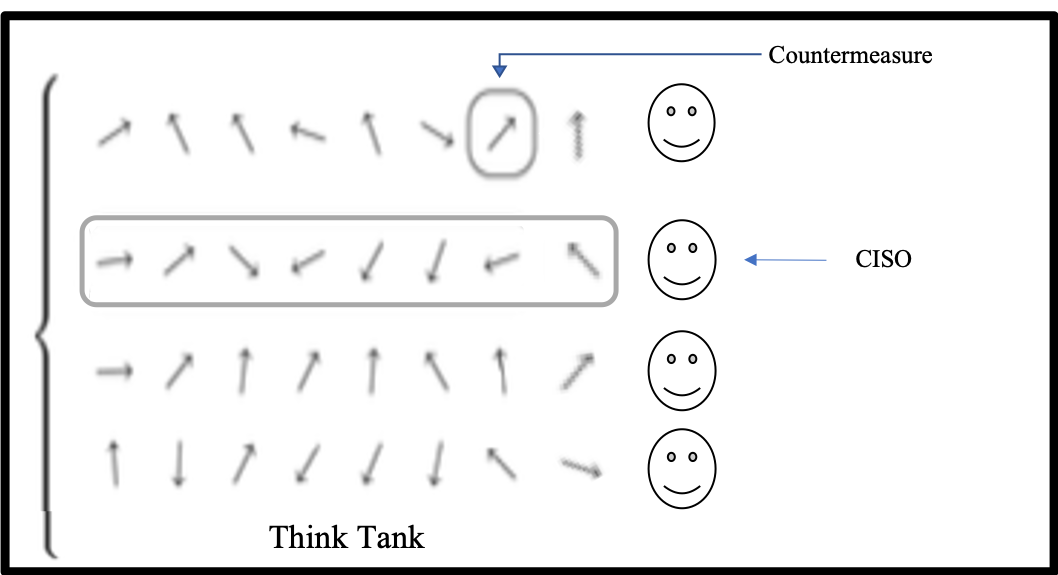
\includegraphics[width=10cm,height=5cm]{Images/quantum-population.png}
\caption{Quantum Population on Q32}%
\end{figure}
\addcontentsline{toc}{subsubsection}{Figure 7: Quantum Population on Q32} 


\vspace{1mm}

After the quantum population is created, each qubit register in that population is initialized with a linear superposition of states. By starting out with an equal chance of getting one and zero, there is natural variability in the population and the genetic algorithm can be more effective. In the case of the cyber security application, the linear superposition of states that the quantum population is initialized with represents an equal probability of a defender implementing a certain control and not implementing that control. Therefore, there is natural variability in the population and the genetic algorithm is effective.

\subsection*{\color{SubSectionBlue}{Phase 2 of Quantum Save}}
\addcontentsline{toc}{subsection}{Phase 2 of Quantum Save} \\

Now that the population has been created and has been initialized with a linear superposition, the second section of the quantum genetic algorithm can begin. This section the individuals with the best random attributes are chosen and the fittest individuals in the population, or those who pack the knapsack the best, will remain for the next generation. After the initialization of the quantum population, it will be classically measured by collapsing the existing wave function. Depending on the alpha and beta values present in each qubit register, a binary string of size two, either 00, 01, 10 or 11, will be obtained from each register 

\begin{algorithm}
\caption{Quantum Save -- Phase 2}
\begin{algorithmic}[1]
\State $CISO \gets 0$
\While{$CISO < \text{4}$}
        \State $binaryString \gets \text{""}$
        \State $result \gets \text{""}$
        \While{$result \text{ in job}$}
            \State $binaryString \gets binaryString + \text{Most Frequent String}$
        \EndWhile
        
        \State $countermeasure \gets 0$
        \State $knapsack \gets 0$
        \While{$countermeasure \text{ in binaryString}$}
            \State $knapsack \gets knapsack + countermeasure$
            \If{$knapsack > b$}
                \State $knapsack \gets knapsack - countermeasure$
            \EndIf
            \State $profit \gets \text{amount saved[}countermeasure\text{]}$
        \EndWhile
        \State $bestIndividual \gets max(profit)$
\end{algorithmic}
\end{algorithm}
\addcontentsline{toc}{subsubsection}{Algorithm 3: The Second Phase} 

During each fitness evaluation, or the conversion between quantum and classical states, the qubit register is measured 1024 times and the most consistent binary string is returned. The binary strings from every four registers will then be combined until four classical strings are obtained, one for each individual in the Think Tank. 

\vspace{1mm}

After quantum measurement, using the Copenhagen interpretation, is complete, the binary strings are evaluated in order to determine the best individual. Depending on the binary string, which essentially represents the controls that are implemented by the defender, a certain mitigation will be received. In this case, if there is a 1 that means that the defender chose to implement a specific control. On the other hand, if there is a zero, then the defender didn’t implement a certain control. Apart from the profit value, a total weight for the knapsack was also obtained, or the total cost of implementing all of the controls, and that total cost was compared to the cost cap, or the budget, set before the first generation. After each binary string is evaluated, the binary string, and respective individual, with the highest profit value is stored as the best chromosome. With the application to a cyber security investment problem, the best chromosome will be the defender that implemented the controls that resulted in the greatest mitigation of the attack.

\subsection*{\color{SubSectionBlue}{Phase 3 of Quantum Save}}
\addcontentsline{toc}{subsection}{Phase 3 of Quantum Save} \\

Since the best strategy to mitigate an attack on the defender’s small-medium enterprise has been determined, the probability amplitudes of each qubit register will be manipulated in the following manner.

\begin{algorithm}
\caption{Quantum Save -- Phase 3}
\begin{algorithmic}[1]
\State $binaryArray \gets binaryString.split()$
\State $CISO \gets 0$
\While{$CISO < 4$}
    \State $countermeasure \gets 0$
    \While{$countermeasure \text{ in } binaryArray$}
        \If{countermeasure != bestIndividual}
            \State $probabilityAmplitude \gets \text{manipulate[}probabilityAmplitude\text{]}$
        \EndIf
        \State $probabilityAmplitude \gets probabilityAmplitude$
    \EndWhile
\EndWhile
\end{algorithmic}
\end{algorithm}
\addcontentsline{toc}{subsubsection}{Algorithm 4: The Third Phase} 

Initially, the first binary pair in the best individual will be obtained and depending on the value of that pair, the probability distribution will be normalized to one. On the other hand, all of the other probability amplitudes will decrease by a factor of $probabilityAmplitude$, a hyper parameter in the algorithm. In this case, the probability of a defender implementing the successful controls increases while the probability of a defender implementing the unsuccessful controls decreases. The factor of probability manipulation, $probabilityAmplitude$, is a hyper parameter of this algorithm and this hyper parameter was tuned by testing out different values for and observing the optimization of the knapsack problem. In the end, the controls that resulted in higher mitigation of an attack were encouraged while controls that resulted in lower mitigation of an attack were discouraged (Fig 8).

\begin{figure}[ht]%
\centering
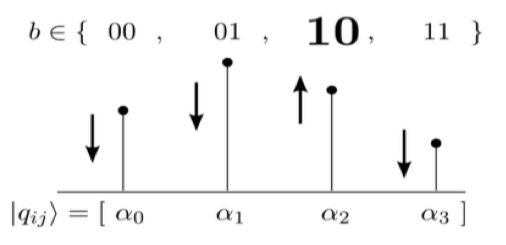
\includegraphics[width=10cm,height=5cm]{Images/amplitude-man.png}
\caption{Manipulation of Probability Amplitudes}%
\end{figure}
\addcontentsline{toc}{subsubsection}{Figure 8: Manipulation of Probability Amplitudes} 

At this point, the algorithm has completed one generation of fitness evaluations. In order to obtain an accurate optimization of the knapsack problem, this process needs to be repeated for 10 generations in order to get a higher optimization of the knapsack problem. At the end of these ten generations, the data of final profit outputted by Quantum Save will be obtained and that data can be compared to that of previous research. However, now that the probability amplitude manipulation is complete and the optimal value has been determined, a disaster algorithm will be implemented. In this case, the disaster algorithm will simply reset the population to a linear superposition of states in the middle of Quantum Save. However, the generation that the disaster algorithm is implemented, is a hyper parameter of this algorithm and this hyper parameter was tuned by testing out different generations. In the end, the location of the disaster algorithm was chosen by the overall mitigation of an attack by the defender.

\vspace{1mm}

After one instance of the algorithm, or 10 generations, has completed its run-time, the data of final profit outputted by Quantum Save will be obtained and that data will be compared to that of previous research. On top of that, the different hyper parameters including the value and the generation for the disaster algorithm will be tuned.

\subsection*{\color{SubSectionBlue}{Why Quantum Computing}}
\addcontentsline{toc}{subsection}{Why Quantum Computing} \\

With this quantum algorithm, one important aspect is the evolution of the population. In order for a population to evolve, there needs to be random variation in the population so that certain traits emerge over others. If every generation contained the same traits, then the entire population would either die or survive. Instead, mutations and gene crossovers drive the idea behind natural selection. With this evolution process, a quantum computer would significantly enhance the effect of a genetic algorithm. \newpage

\begin{figure}[ht]%
    \centering
    \subfloat[General Qubit Properties]{{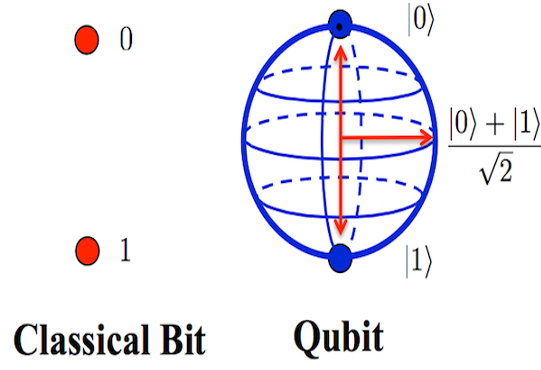
\includegraphics[width=6cm]{Images/qubit.png} }}%
    \qquad
    \subfloat[IBM Quantum Simulator]{{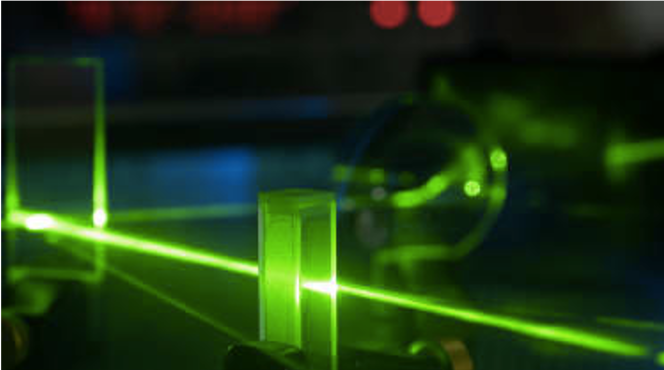
\includegraphics[width=5cm]{Images/ibm_q.png} }}%
    \caption{Power of the Qubit}%
    \label{fig:example}%
\end{figure}
\addcontentsline{toc}{subsubsection}{Figure 9: Power of the Qubit} \\

On a traditional classical computer, a bit is isolated to either 0 or 1, but a qubit uses quantum mechanical properties to simulate a weighted probability distribution between 0 and 1. Each qubit is initialized with a 50\% chance of returning 1 and a 50\% chance of returning 0. As the algorithm progresses, the probabilities change, with a potential 90\% chance of returning 1 and a 10\% chance of returning 0. In a classical genetic algorithm, random variation is controlled by unique constants. However, by using quantum computing, the random variation is inherent within the computational method. The measurement value of a qubit is never concrete but fluctuates based upon probability amplitudes. More specifically, the IBM quantum simulator uses a dilution refrigerator to suspend an electron and shoot a pulse at the suspended electron. If the electron is spin-up, the qubit returns a zero. On the other hand, if the electron is spin-down the qubit returns a one. This allows the IBM Q32 simulator to accurately simulate a quantum state.








